% !TEX root = SystemTemplate.tex

\chapter{Design  and Implementation}
The Dahl Virtual Museum project will be done entirely in the Unreal Engine 4.0 using the built in Blueprint system (a visual scripting IDE).  Any code that will have to be written will be done in C/C++ and integrated into the Blueprint system.  

This section will detail the different aspects of the Blueprints that will constitute the code of this project.  There will be screenshots of the blueprints of each aspect of the project, which are: movement(free and on-rails), the room, the paintings, text descriptions, and alternate environments. 
 

\section{Movement }

\subsection{Technologies  Used}
Unreal Engine 4.0 Blueprint system

\subsection{Component  Overview}
\begin{enumerate}
\item Free movement
\item On-rail movement
\end{enumerate}

\subsection{Phase Overview}
This component was finished in phase 1, during sprint 3. 

\subsection{ Architecture  Diagram}
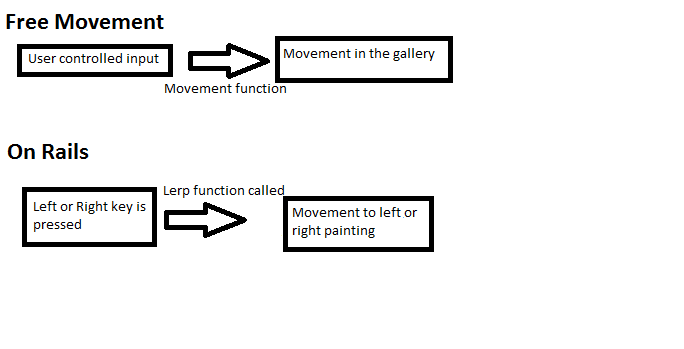
\includegraphics[scale=1.0]{Diagrams/MovementDiagram.png}


\subsection{Data Flow Diagram}
It is important to build and maintain a data flow diagram.  However, it may be 
that a component is best described visually with an architecture diagram. 


\subsection{Design Details}
%This is where the details are presented and may contain subsections.   
Movement is a very crucial piece of this project, which is the reason there was two different methods developed.  Both methods were beta tested by multiple people and showed that they were very much on track of what is required. 




\section{Paintings }

\subsection{Technologies  Used}
Unreal Engine 4.0 Blueprint system

\subsection{Component  Overview}
\begin{enumerate}
\item Paintings were received as .jpg files
\item Image files then converted to .png
\item Drag and drop .png files onto objects in Unreal editor
\end{enumerate}

\subsection{Phase Overview}
I'm not exactly sure what to put for this or any of the phase overviews 

\subsection{ Architecture  Diagram}
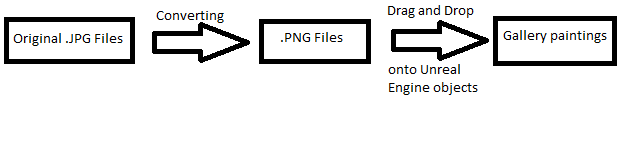
\includegraphics[scale=1.0]{Diagrams/PictureDiagram.png}
 


\subsection{Design Details}
This was a tedious process due to the fact that every file had to be converted from .jpg to .png in order for them to work in the engine.  Then was the task of making the objects in the right dimension for each painting which was done by making box objects to scale with the width and height of each painting, then dragging the .png file onto the object itself thereby creating the texture.


\section{Gallery }

\subsection{Technologies  Used}
Unreal Engine 4.0
Measuring Tape

\subsection{Component  Overview}
The gallery itself was fairly easy to generate.  A blueprint of the actual room was provided by the Dahl and make rendering the Unreal Engine as simple as make the right sized objects.  The four outer walls were very easy to generate from the blueprint, the two protruding walls had to be measured by hand. The rounded corners however were more difficult to recreate because there are no rounded walls in the Unreal Engine, so they had to be custom made.  

\subsection{Phase Overview}
This is an extension of the Phase Overview above, but specific to this component. 
 It is meant to be basically a brief list with space for marking the phase status. 

\subsection{ Architecture  Diagram}
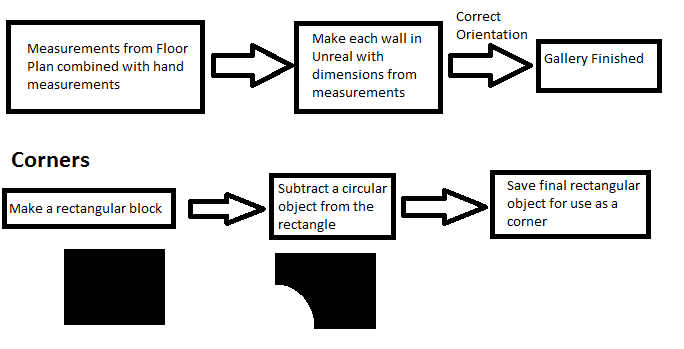
\includegraphics[scale=1.0]{Diagrams/GalleryDiagram.png}


%\subsection{Data Flow Diagram}
%It is important to build and maintain a data flow diagram.  However, it may be 
%that a component is best described visually with an architecture diagram. 


\subsection{Design Details}
This section is about how the actual room was recreated in the Unreal Engine.  The Dahl provided a blueprint of the room which gave the dimensions and angles of the corners which was helpful in mapping it into the engine.  A measuring tape was used for the standalone walls that protrude into the room and the measurements were then scaled to the Unreal Engine unit system.

